\shorthandoff{'}
\begin{markdown*}{%
  hybrid,
  definitionLists,
  footnotes,
  inlineFootnotes,
  hashEnumerators,
  fencedCode,
  citations,
  citationNbsps,
  pipeTables,
  tableCaptions,
}

\chapter{Jaculus-link}

As described in ((TODO)), the communication between the device and the host is done through a single stream connection.

Because the services running on the device work mostly independently, communicating with each service independently is desirable; this is achieved by multiplexing multiple channels on a single stream connection.

Sometimes, the device may have multiple communication interfaces, which can be used for communication with the host. In such cases, it is desirable to be able to route the communication to the appropriate interface.

This functionality is implemented in the Jaculus-link library, which provides a way to multiplex 256 channels on a single stream connection and to route the communication to the appropriate interface. The library is implemented strictly using only C++ 20 standard library for easy portability. For this reason, it does not provide an implementation for communication interfaces, and the user must provide one themselves.

\section{Architecture}

The model of Jaculus-link is split into three layers:

1. Data link layer
2. Routing layer
3. Communicator layer

\subsection{Data link}

The data link is responsible for transmitting data along with channel identifiers. The data link provided in this library is implemented in the `Mux` class, which multiplexes 256 channels on a single stream connection.

It is possible to use other data link implementations as long as they implement the `DataLinkTx` interface for transmission and provide a way to connect them to a `DataLinkRx` for processing received data.

\subsection{Routing layer}

The routing layer is responsible for routing received data to the consumer of the channel. The routing layer is implemented in the `Router` class.

A `Router` instance can be connected to multiple data links and will route data from all of them to the appropriate consumer with the information about the link it was received from. It also allows sending data to a specific link and channel.

\subsection{Communicator layer}

The communicator layer is used as an abstraction layer for communicating through channels. Typically, the communicator is associated with a single channel and provides either an interface for sending or receiving data.

Communicators used for receiving data from a `Router` must implement the `Consumer` interface, which allows them to be subscribed to a specific channel on a `Router` instance. They must process the received data without blocking, preferably only by storing the data in a buffer and processing it later.

Communicators that send data do not have a unified binding interface. Instead, they access the `Router` instance directly and send data to a specific channel on a specific link (or links).

\subsection{Full Jaculus-link pipeline}

The default configuration of the full pipeline provided by the library is shown in the diagram in Figure \ref{fig:link-pipeline}.

\begin{figure}[!ht]
    \centering
    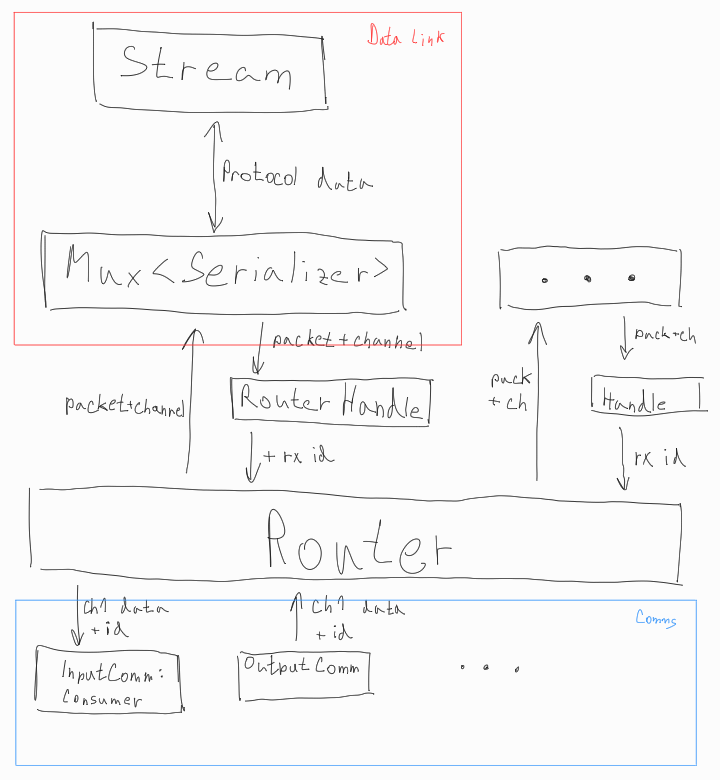
\includegraphics[width=\textwidth]{img/link-pipeline}
    \caption{Default configuration of full Jaculus-link pipeline}
    \label{fig:link-pipeline}
\end{figure}


\section{Multiplexer protocol}

The library provides one protocol for the multiplexer in the class `CobsEncoder`. The protocol is based on a modified version of the COBS\cite{cobs} algorithm for data framing and was originally proposed\footnote{The discussion can be found at \url{https://github.com/yaqwsx/Jaculus/pull/15}.} by Jaroslav Malec for the use in the predecessor version of the Jaculus project.

In the original COBS algorithm, a delimiter byte --- typically zero --- is inserted at the end of the data frame. To encode the transmitted data, every occurrence of the delimiter byte in the data is replaced by a value, that represents the number of bytes to the next delimiter byte. This allows for data framing with a fixed two-byte overhead while limiting the maximum data size to 254 bytes.

The modified version of the algorithm moves the delimiter byte to the start of the data frame and adds length information to the second byte of the data frame. The rest of the data frame is encoded in the same way as in the original algorithm, except for the missing delimiter byte at the end of the data frame, which is only implied by the data frame length. Every such data frame has a three-byte overhead and can contain up to 254 bytes of data. Moving the delimiter byte to the start of the data frame allows for resetting the packetization state in case a previous data frame is lost, malformed, or other corrupted data is received on the stream.

Figure \ref{fig:cobs-diagram} shows a data frame structure diagram. In the data section of the data frame, the first byte contains the channel identifier, followed by the transmitted data. The last two bytes of the data frame contain the CRC16 checksum of the data section.


\begin{figure}[!ht]
    \centering
    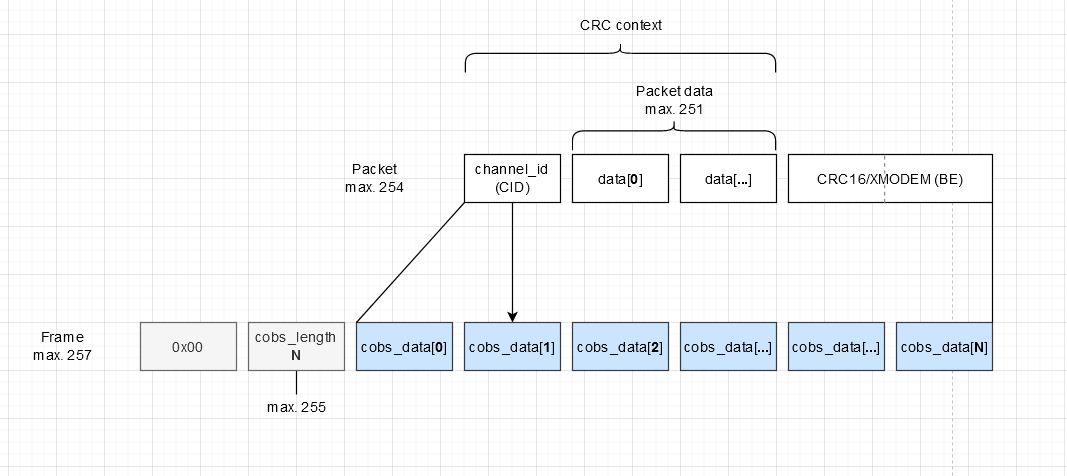
\includegraphics[width=\textwidth]{img/cobs-diagram}
    \raggedright
    \footnotesize{Adapted from: MALEC, Jaroslav. *Protocol diagram*. In: GitHub \[online\]. 2021 \[visited on 2023-05-10\]. Available from: \url{https://github.com/yaqwsx/Jaculus/pull/15}.}
    \caption{Diagram of the COBS-based multiplexer protocol}
    \label{fig:cobs-diagram}
\end{figure}


\section{Usage}

\subsection{Adding the library to a project}

Jaculus-link is a header-only library, so it is sufficient to add the `include` directory to the include path of the project. The library is also configured as a CMake project and exports a target `jac-link` that can be linked to other projects.

\subsection{Multiplexer}

The class `Mux` is a data link implemented as a multiplexer and is templated on the type of the underlying multiplexer protocol. The only protocol provided with the library is in the `CobsEncoder` class. To implement another protocol, the user can create a class with the same interface as `CobsEncoder`.

The `Mux` constructor takes a `Duplex` instance, which serves as an abstraction around the stream connection.

\subsection{Router}

The `Router` class implements the routing layer.

A `Router` instance can be connected to multiple data links as shown in the following example:

```cpp
// Create a router
Router router;

// Create a stream connection
auto stream = std::make_unique<MyStream>();

// Configure a data link
Mux<CobsEncoder> mux(std::move(stream));

// Connect the data link to the router
auto handle = router.subscribeTx(1, mux);
mux.bindRx(std::make_unique<decltype(handle)>(std::move(handle)));
```

The `handle` object is used to receive data from the data link and must be bound to the same data link instance as the one used to subscribe to the router, as it adds the information about the data link to the received data.

\subsection{Communicators}

The communicators are used as an abstraction layer for communicating through channels. Communicators provide an interface for sending or receiving data through a channel.

The provided communicator types are:

- `OutputStreamCommunicator` --- sends data as a stream of bytes
- `InputStreamCommunicator` --- receives data as a stream of bytes
- `OutputPacketCommunicator` --- sends data while exposing the underlying data framing
- `InputPacketCommunicator` --- receives data while exposing the underlying data framing

These communicator types are only interfaces, and their implementations for `Router` are provided in classes with the same names prefixed with `Router`.

The following example shows how to create a pair of stream communicators:

```cpp
Router router;

// Create an input stream communicator
RouterInputStreamCommunicator input({});

// Subscribe the communicator to the router
router.subscribeChannel(1, input);

// Create an output stream communicator and connect it to the router
RouterOutputStreamCommunicator output(router, 1, {});
```


\shorthandon{'}
\end{markdown*}
